\documentclass[a4paper,11pt]{jsarticle}


% 数式
\usepackage{amsmath,amsfonts}
\usepackage{bm}
% 画像
\usepackage[dvipdfmx]{graphicx}
\usepackage{wrapfig}
\usepackage{listings,jvlisting}

\lstset{
  basicstyle={\ttfamily},
  identifierstyle={\small},
  commentstyle={\smallitshape},
  keywordstyle={\small\bfseries},
  ndkeywordstyle={\small},
  stringstyle={\small\ttfamily},
  frame={tb},
  breaklines=true,
  columns=[l]{fullflexible},
  numbers=left,
  xrightmargin=0zw,
  xleftmargin=3zw,
  numberstyle={\scriptsize},
  stepnumber=1,
  numbersep=1zw,
  lineskip=-0.5ex
}

\begin{document}

\title{画像実験課題4}
\author{1029323422 天野岳洋}
\date{\today}
\maketitle
\clearpage

\section{概要}
MNIST のテスト画像 1 枚を入力とし, 3 層ニューラルネットワークを用いて, 0~9の
値のうち1つを出力するプログラムを作成せよ. という課題である.
これは課題3までの内容のみで構成できるため, 非常に簡単に説明を行う.
ただし, 注意したいのは3層NNの入力は, テスト画像1枚が入力なので, 
バッチ単位で扱っていないことである.
\section{実装}
実際のコードを示す.
\begin{lstlisting}
  import numpy as np
  import mnist
  import matplotlib.pyplot as plt
  from pylab import cm
  #load
  parameters = np.load("parameter.npz")
  W1 = parameters['arr_0']
  W2 = parameters['arr_1']
  b1 = parameters['arr_2']
  b2 = parameters['arr_3']

  M = 80
  C = 10
  X = mnist.download_and_parse_mnist_file("t10k-images-idx3-ubyte.gz")

  print("1~9999")
  string_idx = input()
  idx = int(string_idx)

  #show image
  plt.imshow(X[idx], cmap=cm.gray)
  plt.show()

  before_conv = np.array(X[idx])
  img_size = before_conv.size
  img = before_conv.reshape(img_size, 1)

  input1 = np.dot(W1, img) + b1
  output1 = vsigmoid(input1)
  input2 = np.dot(W2, output1) + b2
  alpha = input2.max()
  sumexp = np.sum(np.exp(input2 - alpha))
  output_last = np.exp(input2 - alpha) / sumexp

  answer = np.argmax(output_last)
  print("expected:", end = "")
  print(answer) 
\end{lstlisting}
この3NNが予測した数はソフトマックス層が出力した10個の値の
中で最大値をとるもののargであるから, それを出力する.

\section{実際の動作}
\begin{lstlisting}[caption=Actual Move]
  1~9999
  10
  expected:0
  1~9999
  100
  expected:6
\end{lstlisting}
\begin{wrapfigure}{l}[0pt]{0.5\textwidth}
  \centering
      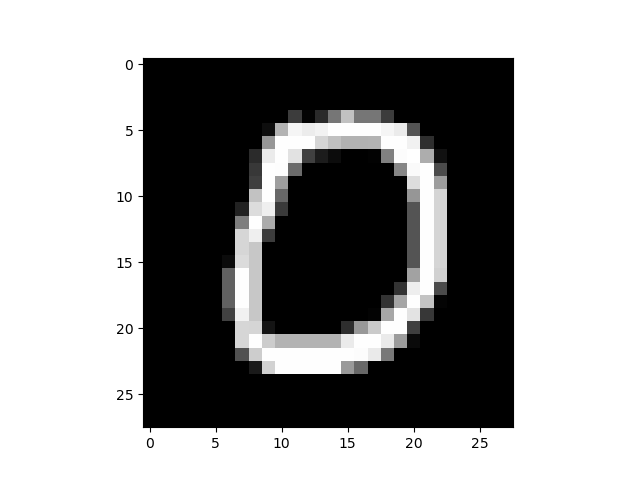
\includegraphics[height = 5cm]{Figure_1.png}
      \centering
        \caption{index=10}
\end{wrapfigure}

左の画像は, 10を入力した時の出力であり, 10番目の画像を表示しており,
その画像に対して予測値は0を出力している. これを計10回行い, 
すべての予測値が正しいことを確認した.
\end{document}